\documentclass[11pt,a4paper]{article}

\usepackage[utf8x]{inputenc}   % omogoča uporabo slovenskih črk kodiranih v formatu UTF-8
\usepackage[slovene]{babel}    % naloži, med drugim, slovenske delilne vzorce
\usepackage{url}
\usepackage{graphicx}



\title{Vmesno poročilo pri predmetu Grafično oblikovanje \\
\large Izdelava promocijskega materiala za potrebe FRI}
\author{Vid Čufar, 63150076 \\
Jernej Habjan, 63150106  \\
Matic Vrtačnik, 63150317 \\
\ \\
Fakulteta za računalništvo in informatiko Univerze v Ljubljani
\date{\today}         
}


\begin{document}
\maketitle


\section{Izbira in raziskava področja teme}
S skupino smo se odločili, da bomo oblikovali majico za promocijske namene FRI. Ker je fakulteta bolj znanstveno naravnana, smo razmišljali o uporabi šal povezanih s programiranjem v oblikovanju našega izdelka. Najprej smo si vzeli nekaj časa in zbrali različne vrste primernih šal z raznih internetnih forumov. Tukaj je prevladovala predvsem stran Stack Overflow, ki je zelo poznana v svetu programiranja in je tako vsebovala vprašanje povezano z našo zastavljeno temo. Povezavo nanj lahko najdemo v viru \cite{jokesource} in vsebuje mnogo strani raznih programerskih šal in kratkih zgodb. 


\section{Opis izbrane teme}
Po izboru najboljših šal, smo se skupaj odločili za tisto, ki se nam je zdela najbolj primerna in izvirna. Najprivlačnejša izbira se nam je zdela preprosta slika, ki jo lahko najdemo na strani v viru \cite{jokesource} med najbolje uvrščenimi odgovori in prikazuje starejšo verzijo avtomobila Volkswagen hrošč, ki ima na registrski tablici napis "FEATURE" (glej sliko \ref{sl:feature}) , ki v opisanem kontekstu ponazarja šalo, da pri programski opremi ne gre za napako ampak za uporabno funkcionalnost. 

\begin{figure}[htb]
\centerline{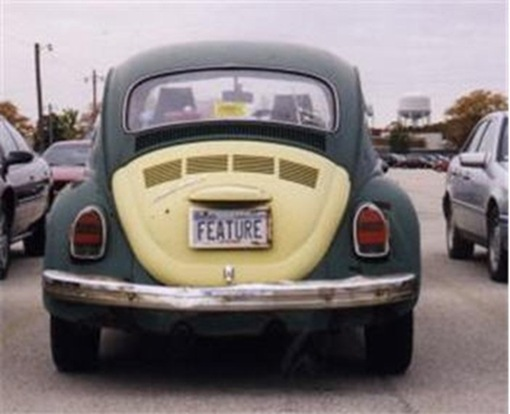
\includegraphics[scale=0.5]{feature.jpg}}
\caption{Slika Volkswagnovega hrošča, ki predstavlja motivacijo oblikovanja našega koncepta.}
\label{sl:feature}
\end{figure}


\section{Koncept izdelave}
Po uspešnem izboru teme smo se nato lahko lotili izdelave koncepta našega izdelka. Najprej smo na internetu našli primerno sliko Volkswagnovega hrošča in jo v silhuetnem načinu v Adobovem Illustratorju obrisali ter dodali primeren tekst, ki skupaj z obrisom izrazi izbrano šalo. Zamislili smo si, da bi bil lahko tak koncept slike s tekstom (vidno na sliki \ref{sl:koncept}) natisnjen na sredini na sprednjem delu majice, na zadnjem pa bi bil na sredini zgoraj logotip FRI. Najverjetneje bi šlo za majico temnejše barve in bi tako lahko uporabili negativ slike \ref{sl:koncept} na sprednjem delu majice.

\begin{figure}[htb]
\centerline{
\includegraphics[width=1.0\textwidth, scale = 0.5]{koncept.png}}
\caption{Trenutna različica našega koncepta majice.}
\label{sl:koncept}
\end{figure}


\bibliographystyle{plain}
\bibliography{literatura}

\end{document}  




